\section{Considere un sistema mecánico descrito por la ecuación.
\begin{equation*}
y''+\frac{1}{4}y'+2y=2cos(\omega t)
\end{equation*}
$y(0)=0, y'(0)=2$, encuentre la solución al problema de valores iniciales y use algún software para graficar la solución.}

Tenemos que la ecuación homogénea esta dada por
\begin{equation*}
y''+\frac{1}{4}y'+2y=0
\end{equation*}
Entonces proponemos lo siguiente
$$y=e^{rt}$$
$$y'=re^{rt}$$
$$y''=r^2e^{rt}$$
Sustituimos en la EDO.
$$r^2e^{rt}+\frac{1}{4}re^{rt}+2e^{rt}=0$$
$$(r^2+\frac{1}{4}r+2)e^{rt}=0$$
$$r^2+\frac{1}{4}r+2=0$$
Resolvemos la ecuación; multiplicamos por $4$ ambos lados de la ecuación $$r^2+\frac{1}{4}r+2=0$$ obtenemos $$4r^2+r+8=0$$ entonces,
$$r=\frac{-1 \pm \sqrt{1^{2}- 4(4)(8)}} {2(4)}$$
$$r=\frac{1 \pm \sqrt{127}i}{8}$$
$$r_{1}=- \frac{1}{8}+ \frac{\sqrt{127}i}{8}$$
Pero tenemos que
$$r=a+bi$$
$$y=e^{at}(C_1cos(bt)+C_2isen(bt))$$
Por lo cual, la solución de la homogénea es
$$y=e^{-\frac{1}{8}t}(C_{1}cos(\frac{\sqrt{127}}{8}t)+C_{2}sen(\frac{\sqrt{127}}{8}t))$$
Ahora buscamos la solución particular de
\begin{equation*}
y''+\frac{1}{4}y'+2y=2cos(\omega t)
\end{equation*}
Notemos que
$$2cos(\omega t)=cos(2e^{i \omega t})$$
Con lo cual podemos resolver la EDO que queda de la siguiente manera
\begin{equation*}
y''+\frac{1}{4}y'+2y=2e^{i \omega t}
\end{equation*}
Proponemos una solución particular
$$y=Ae^{i \omega t}$$
$$y'=Ai \omega e^{i \omega t}$$
$$y''=-A \omega^2 e^{i \omega t}$$
Sustituimos en la EDO, tenemos que
$$-A \omega^2 e^{i \omega t}+\frac{1}{4}Ai \omega e^{i \omega t}+2Ae^{i \omega t}=2e^{i \omega t}$$
$$Ae^{i \omega t}(-\omega^2+\frac{1}{4}i\omega+2)=2e^{i \omega t}$$
entonces
$$A= \frac{2}{(-\omega^2+\frac{1}{4}i\omega+2)} \cdotp \frac{(-\omega^2-\frac{1}{4}i\omega+2)}{(-\omega^2-\frac{1}{4}i\omega+2)}=\frac{2(-\omega^2-\frac{1}{4}i\omega+2)}{(-\omega^2+2)^2-\frac{1}{16}\omega^2}$$
$$A=\frac{2(-\omega^2+2)}{(-\omega^2+2)^2-\frac{1}{16}\omega^2}-\frac{\frac{2}{4}\omega i}{(-\omega^2+2)^2-\frac{1}{16}\omega^2}$$
Por lo cual tenemos que
$$Im(Ae^{i\omega t})=Re(A)Im(e^{i\omega t})+Im(A)Re(e^{i\omega t})$$
entonces
\begin{equation*}
g(x)=\frac{2(-\omega^2+2)}{(-\omega^2+2)^2-\frac{1}{16}\omega^2} \cdotp sen(\omega t)-\frac{\frac{2}{4}\omega}{(-\omega^2+2)^2-\frac{1}{16}\omega^2} \cdotp cos(\omega t)
\end{equation*}
Por lo tanto, la solución de la EDO queda de la siguiente manera
\begin{equation*}
y_g=e^{-\frac{1}{8}t}(C_{1}cos(\frac{\sqrt{127}}{8}t)+C_{2}sen(\frac{\sqrt{127}}{8}t))+\frac{2(-\omega^2+2)}{(-\omega^2+2)^2-\frac{1}{16}\omega^2}sen(\omega t)-\frac{\frac{2}{4}\omega}{(-\omega^2+2)^2-\frac{1}{16}\omega^2}cos(\omega t)
\end{equation*}
Como la solución de la EDO debe cumplir que $y(0)=0$; y en el caso en que $\omega =0$, entonces tenemos que
$$y_g=0=C_1 \Rightarrow -1=C_1$$
Además, $y'(0)=2$, entonces tenemos
$$y'_g=-e^{-\frac{1}{8}x}(-\frac{\sqrt{127}}{8}C_{1}sen(\frac{\sqrt{127}}{8}t)+\frac{\sqrt{127}}{8}C_{2}cos(\frac{\sqrt{127}}{8}t))+t\frac{2(-\omega^2+2)}{(-\omega^2+2)^2-\frac{1}{16}\omega^2}sen(\omega t)-\frac{\frac{2}{4}\omega}{(-\omega^2+2)^2-\frac{1}{16}\omega^2}cos(\omega t)$$
$$y_g=2=-1-\frac{\sqrt{127}}{8}C_2 \Rightarrow 2+1=-\frac{\sqrt{127}}{8}C_2 \Rightarrow \frac{3}{\frac{\sqrt{127}}{8}}=C_2 \Rightarrow \frac{24}{\sqrt{127}}=C_2$$
Sustituyendo estos valores en la solución general de la EDO llegamos a la solución particular del problema de valor inicial. 
\begin{equation*}
y_p(t)=e^{-\frac{1}{8}t}(-cos(\frac{\sqrt{127}}{8}t)+\frac{24}{\sqrt{127}}sen(\frac{\sqrt{127}}{8}t))
\end{equation*}
La gráfica de la solución es la siguiente:
\\
\begin{figure}[h]
    \centering
    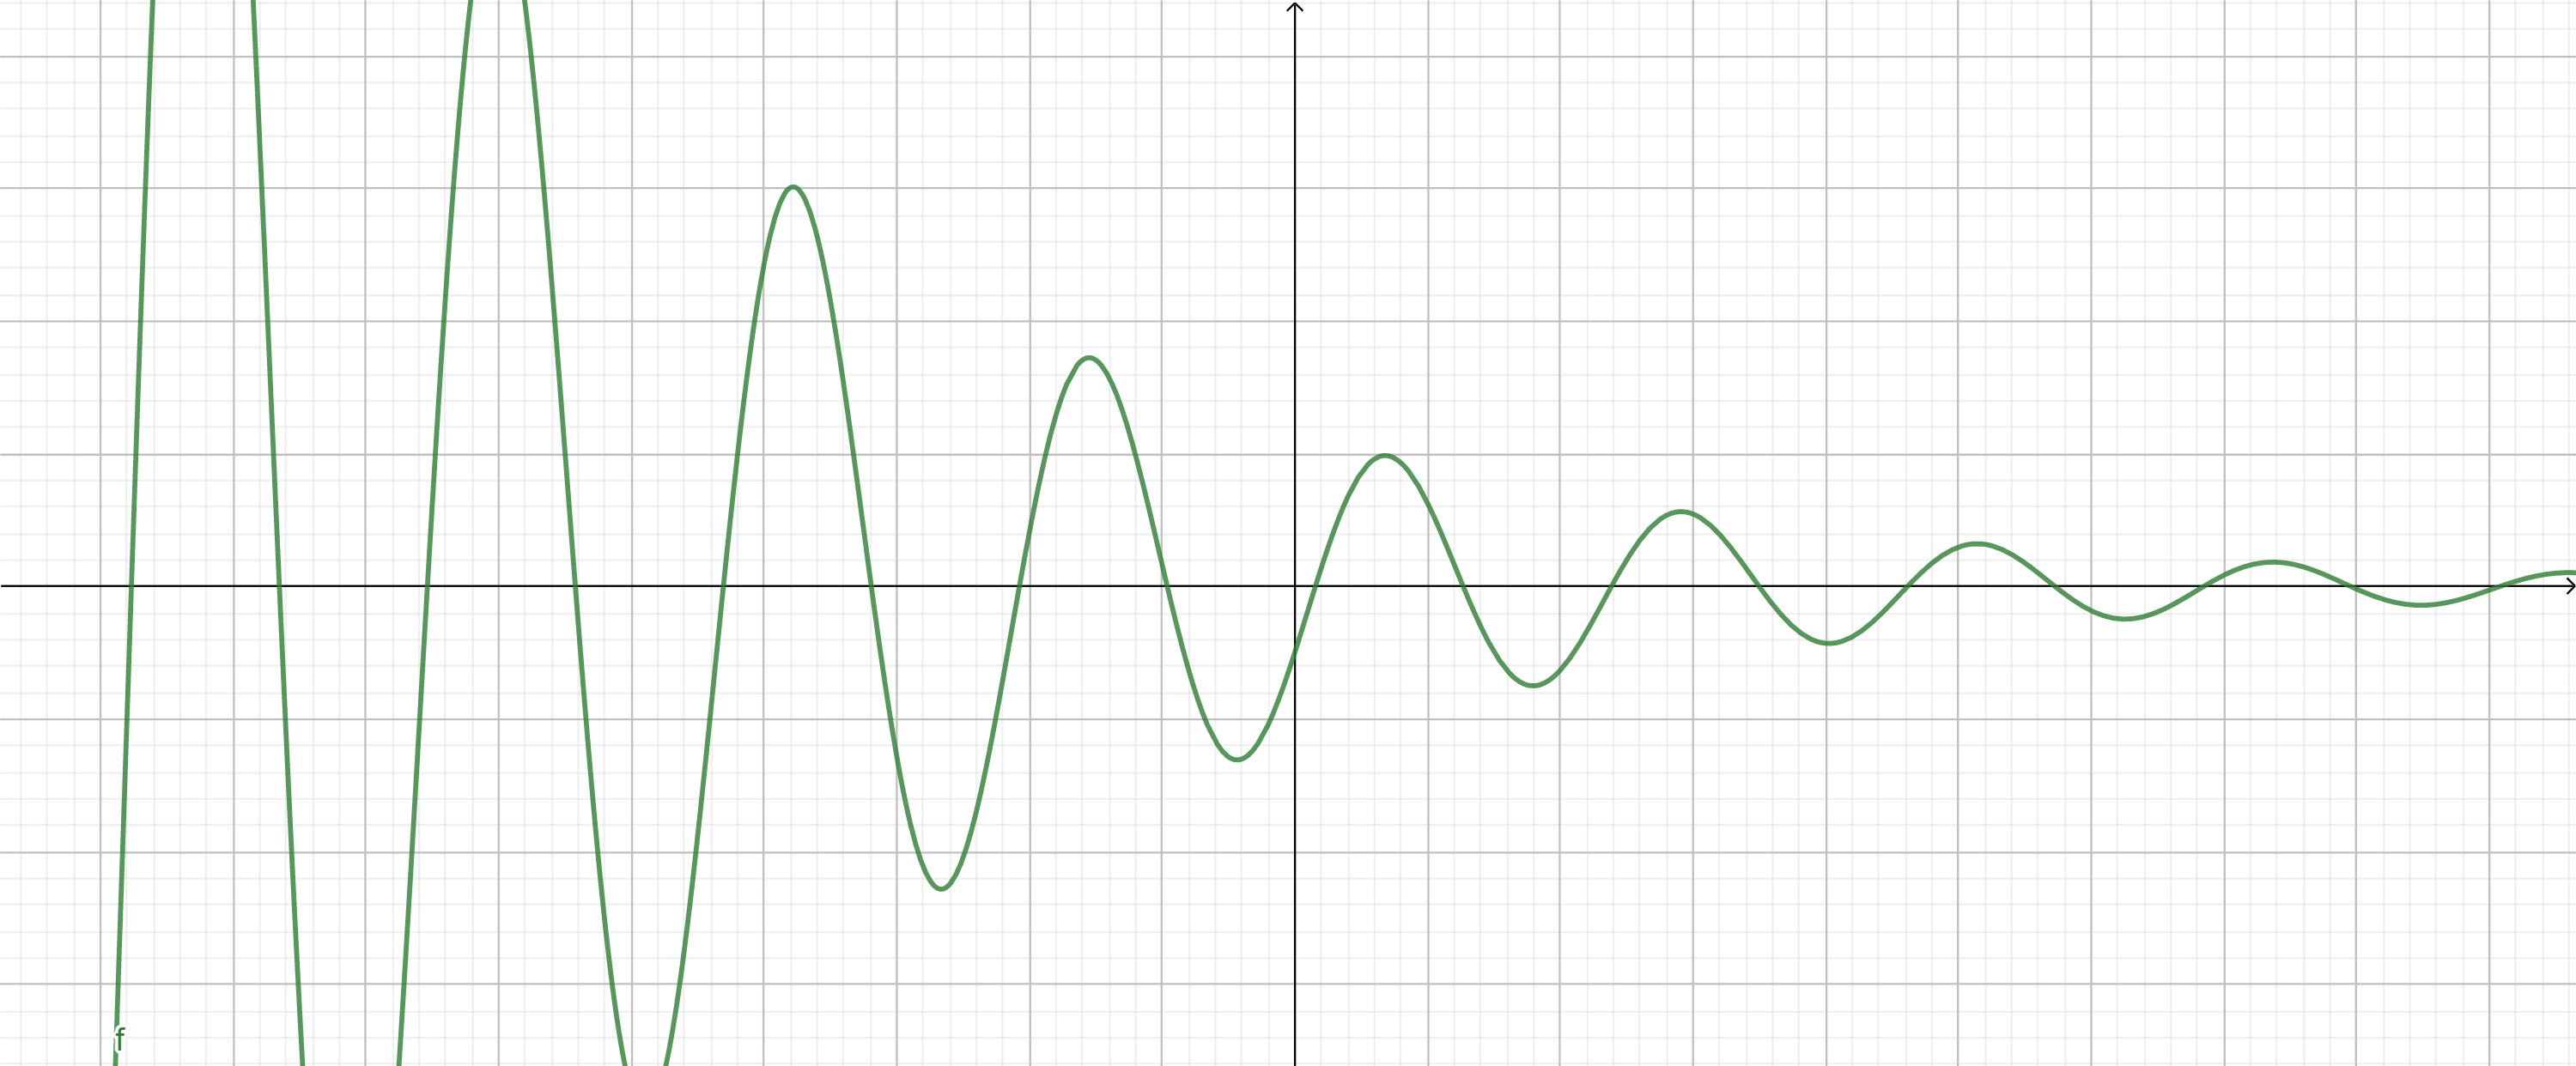
\includegraphics[height = 10cm, width = 15cm]{Ejercicios/Imágenes/ejercicio9.png}
    \caption{Solución de la ecuación del PVI}
\end{figure}